\documentclass[11pt, english]{article}
%\usepackage[latin1]{inputenc}
\usepackage[T1]{fontenc}
\usepackage[utf8]{inputenc}
\usepackage[english]{babel}   % S P R A A K
% \usepackage{graphicx}    % postscript graphics
\usepackage{amssymb, amsmath, amsthm, amssymb} % symboler, osv
\usepackage{mathrsfs}
\usepackage{url}
\usepackage{thmtools}
\usepackage{enumerate}  % lister $  
\usepackage{float}
\usepackage{tikz}
\usepackage{tikz-cd}
\usetikzlibrary{calc}
%\usepackage{tikz-3dplot}
\usepackage{subcaption}
\usepackage[all]{xy}   % for comm.diagram
\usepackage{wrapfig} % for float right
\usepackage{hyperref}
\usepackage{mystyle} % stilfilen      

\usepackage[a5paper,margin=0.5in]{geometry}

\begin{document}
\title{Algebraic groups and moduli theory}
\author{Fredrik Meyer}
\maketitle 

\abstract{
These are notes from the course Algebraic Geometry III. We work over a field of characteristic zero. We start by doing some basic representation theory. Then we introduce algebraic groups. Then we study representations of algebraic groups. Finally we apply this to moduli problems. 
}

\section{Introduction and motivation}

The construction of parameter spaces is central to algebraic geometry. Say you have some class of objects (e.g. isomorphism classes of elliptic curves, quadrics, planes in a vector space) that you want to correspond to the points of some space $S$. To do this, one takes the set of objects and divide out by an equivalence relation. This is very subtle, and the very first question one ask is if this question exists at all.

A good paramter space does not exist for curves of genus $g$ for example. This is essentially because you want a family all of whose fibers are isomorphic to be the trivial family, but because of automorphisms, there are nontrivial families with isomorphic fibers. The problem was solved in the 60's by Mumford and Deligne (and their accomplices) by the introduction of \emph{stacks}, which are generalizations of schemes. This allowed them to define $\ol{\mathfrak M_g}$, a compactification of the moduli space of genus $g$ curves.

The introduction of stacks is somewhat unsatisfactory, however, in that we loose geometry (there are no points).

The quotient is often a quotient by a group action, and this is often an \emph{algebraic} group action. So the situation is this: we have an action $G \curvearrowright X$ of an algebraic group $G$ on some algebraic space $X$. Then we ask when the quotient $X/G$ exists, and if it does, in what sense? The naive approach of taking the points to be the orbits of $G$ does not work as we will see in the examples below.

Let us first consider the affine case. That is, let $X = \Spec A$, where $A$ is some finitely-generated $k$-algebra. What should the space $X/G$ be? First of all, note that an action on $X$ induce an action on $A$: if $f \in A$, then we see that $g \cdot f$ is the function defined by $(g \cdot f)(x)=f(g \cdot x)$ for all $x$. We want functions on $X/G$ to correspond to functions that are constant on $G$-orbits. Thus we are led to consider $A^G$, namely the invariant subring of $A$.

Problem! Even if $A$ is finitely generated, $A^G$ is \emph{usually} not!

We end this section with a collection of examples of what can happen and what can go wrong when studying quotients. First an example where things are good.

\begin{example}
Consider the representation of $\Z_n$ on $\SL_2(\C)$ given by
$$
\Z_n \ni [m] \mapsto 
\begin{pmatrix}
  \zeta_n & 0 \\ 0 & \zeta_n^{-1}
\end{pmatrix} \in \SL_2(\C),
$$
where $\zeta_n$ is an n'th root of unity. The action on the coordinate ring $\C[x,y]$ is given by $x \mapsto \zeta_n x$ and $y \mapsto \zeta_n^{-1}y$. Thus the action on a monomial is given by $x^ay^b \mapsto \zeta_n^{a-b}x^a y^b$. This monomial is invariant if and only if $a \equiv b \pmod{n}$.

Let us plot these monomials for $n=3$: 
\begin{center}
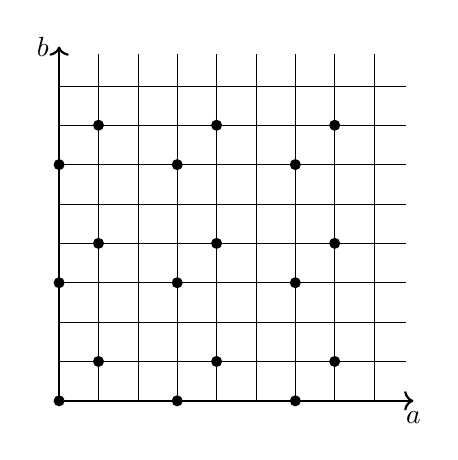
\begin{tikzpicture}
 \draw[step=0.5cm, very thin] (0,0) grid (4.4,4.4);
\draw[thick, ->] (0,0) -- (0,4.5) node[left] {$b$};
\draw[thick, ->] (0,0) -- (4.5,0) node[below] {$a$};

\foreach \x in {0,3,6}
  \foreach \y in {0,3,6} {
    \fill ({0.5*\x},{\y*0.5}) circle (2pt);
    \fill ({0.5*\x+0.5},{\y*0.5+0.5}) circle (2pt);
} 
\end{tikzpicture}
\end{center}

As a semigroup, this is generated by the monomials $x^n,xy$ and $y^n$, so that $\C[x,y]^{\Z_n}=\C[x^n,xy,y^n]=\C[u,v,w]/(uw-v^n)$. This is a toric surface singularity of type $A_{n-1}$.

The  map $\C^2 \to \Spec \C[x,y]^{\Z_n}$ is of degree $n$, since the field extension $\C(x^n,xy,y^n)=\C(x^n,xy) \hookrightarrow \C(x,y)$ is of degree $n$. The only ``bad'' point is the origin, which have only one fiber.
\end{example}

\begin{example}
  Let $G = \C^\ast$ and let $X = \C^n$. Consider the representation
$$
\C^\ast \ni \lambda \mapsto 
\begin{pmatrix}
  \lambda & 0 & \\
0 & \ddots &0 \\
&0 & \lambda
\end{pmatrix} \in \GL_n(\C).
$$

We have an induced action on the coordinate ring, sending $x_i$ to $\lambda x_i$. But the only invariants are the constants! Thus the ``quotient'' is just the constant map $\C^n \to \{p\}$. This is not what we want.

Let us analyze the orbits of $G$. If $x \in \C^n$ is non-zero, then the orbit $G \cdot x$ is the line spanned by $x$ minus the origin. If $x=\vec 0$, then the orbit is just the origin. Thus most orbits are not closed, and we notice that the origin is in the closure of all orbits. 

This suggests a possible solution. If we instead consider $\C^n \bs \{ 0\}$, the orbits are disjoint and closed in the subspace topology.
\end{example}

\begin{example}
Let again $G = \C^\ast$, but consider now the representation given by
$$
\C^\ast \ni \lambda \mapsto 
\begingroup
\renewcommand*{\arraystretch}{0.8}
\begin{pmatrix}
  \lambda & 0& & \ldots \\
0& \lambda & & \\
\vdots & & \lambda^{-1} &0 \\
&&0& \lambda^{-1}  \in \GL_2(\C).
\end{pmatrix}
\endgroup
$$
The action extends to the coordinate ring $R= \C[x,y,z,w]$, and the invariants are $R^G=\C[xz,xw,yz,yw]$. Then $R^G \approx \C[t_1,t_2,t_3,t_4]/(t_1t_4-t_2t_3)$. This is a hypersurface in $\C^4$. 

We have a commutative diagram:
\[
\xymatrix{
\C^4 \ar[d] \ar[dr]^\phi & \\
\Spec R^G \ar@{^(->}[r] & \C^4
}
\]
Here $\phi(x,y,z,w)=(xz,xw,yz,yw)$. Then we look at $\phi^{-1}(0)$. A small calculation reveals that this is the union of the $xy$-plane and the $zw$-plane, intersecting in the origin. The problem here is that the fiber over the origin is $2$-dimensional, whereas all the other fibers are $1$-dimensional. In particular the map is not flat.
\end{example}

\begin{example}
An even more serious problem is that $R^G$ might not be finitely generated. It is difficult to construct examples where this happens, though. Masayoshi Nagata constructed a counterexample as follows: let $\Gr_a^n$ act on $\Aa^{2n}$ (in some specified way) and let $G = \Gr_a^{n-r}$ be a general linear subspace of codimension $r$. He proved that if $r=3$ and $n=16$, then $R=\C[x_1,\cdots,x_n,y_1,\cdots,y_n]^G$ is not finitely generated. See \cite{mckernan_moridream} for a readable account of the counterexample (and related problems).
\end{example}

It turns out that the ``magic'' property we want of an algebraic group is that it is ``linearly reductive'' - a technical property implying that $R^G$ is finitely-generated.

The plan ahead is as follows. The next section will talk loosely about representation theory in general in order for the reader to get a feel for the subject. Section 3 will be about algebraic groups and some examples. Section 4 is longer and is about representations of algebraic groups. This is the technical section where linear reductivity is introduced. 


\section{Representation theory in general}

Let $V$ be a vector space. Briefly, a \emph{representation} of any group $G$ on $V$ is just a group homomorphism $\rho:G \to \GL(V)$.

\begin{example}
The \emph{trivial representation} is given by sending every $g \in G$ to the identity transformation.
\end{example}

\begin{example}
Suppose $G$ is a finite group. Then there is an embedding $G \hookrightarrow S_n$, and every element of $S_n$ can be represented by permutation matrices (that is, matrices $M_g$ such that $Me_i=e_{g(i)}$ for all $g \in G$). This defines a representation of $G$ in $k^n$. 
\end{example}

\begin{example}
Suppose $G$ acts on a (finite) set $X$. Let $V$ be the vector space with basis identified with the elements of $X$. Then $G$ acts on $V$ by linearity: for each $g \in G$, $\rho(g)$ is the linear map sending $e_x$ to $e_{gx}$. Such representations are called \emph{permutation representations}.
\end{example}

A \emph{morphism of representations} $(\rho,V)$,$(\rho',W)$ consists of commutative diagrams
\[
\xymatrix{
V \ar[r]^{\psi} \ar[d]_{\rho(g)}& W \ar[d]^{\rho'(g)} \\
V \ar[r]_{\psi} & W
}
\]
for each $g \in G$. Thus, if $\psi$ is invertible, this says that the linear operators $\rho(s),\rho'(s)$ are similar.

\section{Algebraic groups}

Algebraic groups are group objects in the category of affine varieties. More precisely:

\begin{defi}
\label{defalggrp}
Let $A$ be a finitely generated $k$-algebra. An \emph{affine algebraic group} is a quadruple $(A,\mu_A,\epsilon,\iota)$ where $\mu_A:A \to A \otimes_k A$ (the \emph{coproduct}), $\epsilon:A \to k$ (the \emph{coidentity}), $\iota: A \to A$ (the \emph{coinverse}) are $k$-algebra homomorphisms, satisfying the following conditions:
\begin{enumerate}
\item Coassociativity. The following diagram commutes:
\[
\xymatrix{
A \ar[r]^{\mu_A} \ar[d]_{\mu_A} & A \otimes_k A \ar[d]^{\id_A \otimes \mu_A} \\
A \otimes_k A \ar[r]_{\mu_A \otimes \id_A} & A \otimes_k A \otimes_k A
}
\]
\item The following diagram commutes:
\[
\xymatrix{
 & & k \otimes_k A  \ar[dr]^{\simeq} \\
A \ar[r]^\mu & A \otimes_k A \ar[ur]^{\epsilon \otimes \id_A} \ar[dr]_{\id_A \otimes \epsilon}  & & A \\
 & & A \otimes_k k \ar[ur]_{\simeq}
 }
\]
and is equal to the identity.
\item Coinverse. The following diagram commutes:
\[
\xymatrix{
A \ar[d]^\mu \ar[rr]^\epsilon & & k \ar[d] \\
A \otimes_k A \ar[r]_{\id_A \otimes \iota} & A \otimes_k A \ar[r]_\cdot & A
}
\]
Here the right arrow is the morphism making $A$ a $k$-algebra. The last arrow in the lower sequence is multiplication in $A$.
\end{enumerate}
\end{defi}

\begin{example}
If $G=\GL_n$, then $A=k[T_{ij},\det T]$. Then $\mu_A$ is given by
\[
T_{ij} \mapsto \sum_{h=1}^n T_{ih} \otimes T_{hj}.
\]
The coinverse is given by the usual Cramer's rule. Also $\epsilon(T_{ij})=\delta_{ij}$.
\end{example}

\begin{example}
If $G=\Gr_a=(\Aa^1,+)=\Spec k[X]$, then $\mu_A(X)=X \otimes 1 + 1 \otimes X$. The coidentity is $\epsilon(X)=0$, and the coinverse is $\iota(X)=-X$.
\end{example}

\begin{example}
 Let $A=k[s]$ be the polynomial ring in one variable. This is the coordinate ring of $\Aa_k^1$. We can define 
$$
\mu(s) = s \otimes 1 + 1 \otimes s.
$$
Also, $\epsilon(s)=0$, and $\iota(s)=-s$. 
\end{example}


\begin{defi}
\label{defaction}
An \emph{action} of an affine algebraic group $G = \Spec A$ on an affine variety $X= \Spec R$ is a morphism $G \times X \to X$ defined dually by a $k$-algebra morphism $\mu_R : R \to R \otimes_k A$ satisfying the following two conditions.
\begin{enumerate}
\item  The following diagram is commutative:
\[
\xymatrix{
R \ar[dr]^{\id_R} \ar[r]^{\mu_R} & R \otimes_k A \ar[d]^{\id_R \otimes \epsilon} \\
 & R \simeq R \otimes_k k
}
\]
\item The diagram
\[
\xymatrix{
R \ar[r]^{\mu_R} \ar[d]_{\mu_R} & R \otimes_k A \ar[d]^{\mu_R \otimes \id_A} \\
R \otimes_k A \ar[r]_{\id_R \otimes \mu_A} & R \otimes _k A \otimes_k A
}
\]
\end{enumerate}
\end{defi}


\section{Representations of algebraic groups}

Let $G = \Spec A$ be an affine algebraic group over a field $k$. 

\begin{defi}
 An \emph{algebraic representation of $G$} is a pair $(V,\mu_V)$ consisting of a $k$-vector space $V$ and a $k$-linear map $\mu_V: V \to V \otimes_k A$ satisfying the following two conditions:
 \begin{enumerate}
 \item The diagram
\begin{equation}
\label{eq:algrep1}
\xymatrix{
V \ar[dr]^{\id_V} \ar[r]^{\mu_V} & V \otimes_k A \ar[d]^{\id_V \otimes \epsilon} \\
 & V \simeq V \otimes_k k
}
\end{equation}
is commutative.
\item The diagram
\[
\xymatrix{
V \ar[r]^{\mu_V} \ar[d]_{\mu_V} & V \otimes_k A \ar[d]^{\mu_V \otimes \id_A} \\
V \otimes_k A \ar[r]_{\id_V \otimes \mu_A} & V \otimes _k A \otimes_k A
}
\]
is commutative. Here $\mu_A$ is the coproduct in the coordinate ring of $G$.
 \end{enumerate}
\end{defi}

\begin{remark}
In lieu of Definition \ref{defaction}, we see that any action of an algebraic group $G$ on an affine variety $X=\Spec R$ is a representation of $G$ on the infinite-dimensional $k$-vector space $R=\Gamma(X,\OO_X)$.
\end{remark}

\begin{remark}
Mumford and Fogarty calls this a \emph{dual action of $G$ on $V$}, in their famous ``Geometric Invariant Theory'' \cite{mumford_git}.
\end{remark}

We often drop the subcript from $\mu_V$ unless confusion may arise. The same comment applies to tensor products. They will always be over the ground field unless otherwise stated. We will sometimes refer to a representation $(V,\mu_V)$ sometimes as ``a representation $\mu:V \to V \otimes A$'' and sometimes as just ``a representation $V$''.

\begin{defi}
Let $\mu:V \to V \otimes A$ be a representation of $G = \Spec A$. Then:
\begin{enumerate}
\item A vector $x \in V$ is said to be \emph{$G$-invariant} if $\mu(x) = x \otimes 1$.
\item A subspace $U \subset V$ is called a \emph{subrepresentation} if $\mu(U) \subseteq U \otimes A$. 
\end{enumerate}
\end{defi}

\begin{prop}
\label{propfinite}
Every representation $V$ of $G$ is locally finite-dimensional. Precisely: every $x \in V$ is contained in a finite-dimensional subrepresentation of $G$.
\end{prop}

\begin{proof}
Write $\mu(x)$ as a finite sum $\sum_i x_i \otimes f_i$ for $x_i \in V$ and linearly independent $f_i \in A$. This we can always do, by definition of tensor product and bilinearity. Let $U$ be the subspace of $V$ spanned by the vectors $x_i$. 

Now, by the commutativity of the diagram \eqref{eq:algrep1} it follows that $$ x = \sum_i \epsilon(f_i) x_i. $$

By the commutativity of the second diagram in the definition, it follows that
$$
\sum_i \mu_V (x_i) \otimes f_i = \sum_i x_i \otimes \mu_A(f_i) \in U \otimes A_k \otimes_k A.
$$

Because each term of the right-hand-side is contained in $U \otimes A \otimes A$, it follows that $\mu_V(x_i)$ is contained in $U$ since the $f_i$ are linearly independent.

Thus $x$ is contained in the finite-dimensional representation $\restr{\mu_V}{U}:U \to U \otimes A$.
\end{proof}

We can classify representations of $\Gr_m$ easily. They are all direct sums of ``weight $m$''-representations, that is, representations of the form $$V \to V \otimes k[t, t^{-1}], v \mapsto v \otimes t^m.$$ 

\begin{prop}
\label{propgm}
 Every representation $V$ of $\Gr_m$ is a direct sum $V = \oplus_{m \in \Z} V_{(m)}$, where each $V_{(m)}$ is a subrepresentation of weight $m$. 
\end{prop}

\begin{proof}
For each $m \in \Z$, define
\[
V_{(m)} = \{ v \in V \mid \mu(v) = v \otimes t^m \}.
\]
This is a subrepresentation of $V$: we must see that $\mu(V_{(m)}) \subset U \otimes A$, but this is true by construction. It is also clear that is has weight $m$. Next we show that $V = \oplus_{m \in \Z} V_{(m)}$. Write
\[
\mu(v) = \sum_{m \in \Z} v_m \otimes t^m \in V \otimes k[t,t^{-1}].
\]

Using the first condition in the definition of a representation, we get that $v = \sum_{m \in \Z} \epsilon(t^m)v_m$. It remains to check that each $v_m \in V_{(m)}$ (we can forget the scalars $\epsilon(t^m)$). But from definition ii), it follows that
\[
\sum \mu(v_m) \otimes t^m = \sum v_m \otimes t^m \otimes t^m,
\]
so that indeed $\mu(v_m)= v_m \otimes t^m$, as wanted.
\end{proof}

\begin{example}
An action of $\Gr_m$ on $X = \Spec R$ is equivalent to specifying a grading
\[
\xymatrix{
R = \bigoplus_{m \in \Z} R_{(m)} & R_{(m)}R_{(n)} \subset R_{(m+n)}.
}
\]
The invariants under this action are thus the homogeneous elements of weight zero, that is, the subring $R_{(0)}$. Moreover, we have a special operator. There is a linear endomorphism $E$ of $R$ that sends $f = \sum f_m \mapsto \sum m f_m$, and it is a derivation of $R$, called the Euler operator. We have $R^{\Gr_m}=\ker E$.

To see that $E$ is a derivation, we must check that $E(fg)=fE(g)+gE(f)$. The operator is homogeneous, so it is enough to check on homogeneous elements. So let $f_m,g_n$ be of degree $m,n$, respectively. Then
\[
E(f_mg_n)=(m+n)f_mg_n = g_n(mf_m)+f_m(ng_n)=g_nE(f_m)+f_mE(g_m),
\]
as wanted.
\end{example}


A character is a homomorphism $G \to \C^\ast$, so we have a corresponding notion of characters in this ``dual'' world:

\begin{defi}
Let $G=\Spec A$ be an affine algebraic group. A $1$-dimensional character of $G$ is a function $\chi \in A$ satisfying
\[
\xymatrix{
\mu_A(\chi) = \chi \otimes \chi & \iota(\chi)\chi = 1.
}
\]
\end{defi}

\begin{lemma}
The characters of the general linear group $\GL(n) = \Spec k[x_{ij}, \det X]$ are precisely the integer powers of the determinant $(\det X)^n$ for $n \in Z$.   
\end{lemma}

\begin{defi}
  Let $\chi$ be a character of an affine algebraic group $G$, and let $V$ be a representation of $G$. A vector $v \in V$ satisfying $$\mu_V(v) = v \otimes \chi$$ is called a \emph{semi-invariant} of $G$ with weight $\chi$. The semi-invariants of $V$ belonging to a given character $\chi$ form a subrepresentation $V_\chi \subset V$ of $V$.
\end{defi}

We will often change the point of view depending upon the situation. Sometimes we think of a representation of an algebraic group as a $k$-linear map $V \to V \otimes_k A$ satisfying some axioms, and sometimes we think of a representation as a group $G$ acting on a vector space $V$ in the usual fashion.

\begin{prop}
 Let $\mu: V \to V \otimes_k A$ be a representation of an algebraic group $G$. Let $g \in G(k)$ be a $k$-valued point and $\mm_g \subseteq A$ the corresponding maximal ideal. Denote by $\rho(g)$ the composition
\[
V \xrightarrow{\mu} V \otimes_k A \xrightarrow {\mod \mm_g} V \otimes_k k \simeq V.
\]
Then, if $A=\Gamma(G,\OO_G)$ is an integral domain, a vector $v \in V$ such that $\rho(g)(v)=v$ for all $g \in G(k)$ is a $G$-invariant.
\end{prop}
\begin{proof}
We need to check that $\mu(v)=v \otimes 1$.  First, since $G$ is the spectrum of a finitely generated $k$-algebra, we can write $A$ as $k[y_1,\cdots,y_m]/I$ for some prime ideal $I$. Then the same trick as in the proof of Proposition \ref{propfinite} works. Write $\mu(v)=\sum v_i \otimes f_i$ with $f_i \in A$ for all $i$. Since the composition is the identity, we have that $f_i \equiv 1 \pmod{\mm_g}$ for all $g \in G$. This implies that $f_i-1$ is contained in the Jacobson radical of $A$. But $A$ is an integral domain, so $f_i-1=0$.
\end{proof}
Thus, in a sense, the two notions of $G$-invariance coincides.

\subsection{Algebraic groups and their Lie spaces}

In the spirit of Grothendieck (or maybe the spirit of Newton?\footnote{Or Leibniz, or Lie...}), we will consider infinetesimal neighbourhoods of the identity $e \in G=\Spec A$.

\begin{defi}
 Let $R$ be a $k$-algebra and $M$ an $R$-module. An \emph{$M$-valued derivation} is a $k$-linear map $D:R \to M$ satisfying the Leibniz rule $D(xy)=xD(y) + yD(x)$ for $x,y \in R$.
\end{defi}

The set of $M$-valued derivations is also an $R$-module, denoted by $\Der_k(R,M)$. This is used to define tangent spaces in algebraic geometry as follows: Let $p \in \Spec A=X$ be a closed point. Then we have a local ring $\OO_{X,p}$ and a quotient map $\OO_{X,p} \to \OO_{X,p}/\mm_p \simeq  k$. Then the $k$-module $(\mm_p/\mm_p^2)^\vee$ is called the \emph{Zariski tangent space} of $p \in X$. In fact:
\begin{prop}
\label{propzariski}
We have isomorphisms of $\OO_{X,p}$-modules:
$$ \Der_k(\OO_{X,p},k) \simeq (\mm_p/\mm_p^2)^\vee \simeq \Hom_{k-alg}(\OO_{X,p},k[\epsilon])
$$
\end{prop}
\begin{proof}
We first prove the existence of the first isomorphism.

Send $D \in \Der_k(\OO_{X,p},k)$ to $\restr{D}{\mm_p}$. This is well-defined if $D$ vanishes on $\mm_p^2$. But if $m_1,m_2 \in \mm_p$, then $$D(m_1m_2)=m_1D(m_2)+m_2D(m_1)=0 \in \OO_{X,p}/\mm_p.$$
So the map is well-defined.

We have a map in the opposite direction as well. Let $\ell:\mm_p/\mm_p^2 \to k$ be a linear functional on the $k$-vector space $\mm_p/\mm_p^2$. Define $D_\ell$ to be the $k$-linear map $D_\ell:\OO_{X,p} \to k$ given by
$$
D_\ell(f) = \begin{cases}
0 & \text{if $f \in k$} \\
\ell(f) & \text{if $f \in \mm_p$} \\
0 & \text{if $f \in \mm_p^2$}.
\end{cases}
$$
I know claim that this is a derivation. Write $f,g \in \OO_{X,p}$ as $c+m,c'+m'$ where $c$ is outside the maximal ideal and $m \in \mm_p$. Then
$$
D_\ell(fg)=D_\ell(cc'+cm'+c'm+m'm') = cD_\ell(m')+c'D_\ell(m),
$$
by definition of $D_\ell$.

It is easy to check that these two maps are inverse to each other.

We give an isomorphism between the first and the third module. We begin first by studying the elements of $\Hom_{k-alg}(\OO_{X,p},k[\epsilon])$. As a $k$-vector space, $k[\epsilon] = k \oplus \epsilon k$. Thus every $f \in \Hom_{k-alg}(\OO_{X,p},k[\epsilon])$ can be written as $f = \lambda(f) + \epsilon \delta(f)$. But we have a diagram
\[
\begin{tikzcd}
{}& k \arrow{dr} \arrow{dl} & \\
\OO_{X,p} \arrow{dr} \arrow{rr}{f} & & k[\epsilon] \arrow{dl} \\
 & k  
\end{tikzcd}
\]
Thus $\lambda(f)(x) = x \pmod {\mm_p}  = x(p)$. Thus the ``constant part'' of $f$ is determined by default. Furhermore, since $f$ is an algebra morphism, we must have that
\begin{align*}
  f(xy) &= (xy)(p) + \epsilon \delta(f)(xy) \\
f(x)f(y) &= (x(p)+\epsilon \delta(f)(x))(y(p)+\epsilon \delta(f)(y)) \\
&= x(p)y(p) + \epsilon \left( x(p) \delta(f)(y) + y(p) \delta(f)(x)\right).
\end{align*}
Thus we see that the function $\delta(f):\OO_{X,p} \to k$ is a derivation. We thus have a $k$-linear map $\Hom_{k-alg}(\OO_{X,p},k[\epsilon]) \to \Der_k(\OO_{X,p},k)$ by $f \mapsto \delta(f)$. The inverse map is given by the function $D \mapsto {(x \mapsto x(p) + \epsilon D(x))}$. 
\end{proof}

\begin{remark}
This smells of some kind of Taylor expansion. In fact, this can be used to compute tangent spaces of Hilbert schemes. Let $X \subset \PP^n$ be a projective variety, and $[X] \in \Hilb_{P(t)}$ the corresponding point in the Hilbert scheme. By the above, the set of morphisms $\Spec k[\epsilon] \to \Hilb_{P(t)}$ are in one to one correspondence with the tangent space of $\Hilb_{P(t)}$ at $[X]$. But by the universal property of the Hilbert scheme, this set is in one-one correspondence with the set of flat families $\mathfrak X \to \Spec k[\epsilon]$. But these are classified by global sections of $\mathcal N_{X/\PP^n}$, the normal bundle.
\end{remark}

In fact, the module of derivations is what is called a \emph{corepresentable functor}. There is an $R$-module $\Omega_{R/k}$ such that $\Der_k(R,M)=\Hom_R(\Omega_{R/k},M)$, functorially in $M$. This is the module of \emph{Kähler differentials}.

\begin{example}
We compute the Zariski tangent space of $\SL_n$ at the identity element. Note that $\SL_n=\Spec k[x_{ij}]/(\det X-1)=\Spec R$. Let $I=(\det X-1)$, the principal ideal generated by $\det X-1$. There is an exact sequence
$$
0 \to \Der_k(R,k) \to \Der_k(k[x_{ij}],k) \to \Hom_k(I/I^2,k)
$$
of $R$-modules. The first map is just the pullback of the projection $k[x_{ij}] \to R$. The second map send $D \in \Der_k(k[x_{ij}],k)$ to the restriction $\restr{D}{I/I^2}$. This does not a priori make sense. But since we are considering homomorphisms to $k=R/\mm_e$, it is easy to see that any $D$ vanishes on $I^2$. Thus the Zariski tangent space of $SL_n$ at the identity can be computed as the kernel of the map to the right. The middle term is spanned as a $k$-vector space by $\restr{\dd{}{x_{ij}}}{X=I_n}$, so that we can identify it with $\End(V)$.

Since $I$ is principal, it follows that $\Hom_k(I/I^2,k) \simeq \Hom_k(A,k) \simeq k$. Doing all the identifications, the right map is then given by $D \mapsto \restr{D(\det M)}{I_n}$. A computation gives that $\restr{D(\det M)}{I_n}=\tr M $, so that the kernel is given by the matrices with trace zero.
\end{example}

A derivation is a $k$-linear map vanishing at $\mm_p^2$. The generalization of this are \emph{local distributions}:

\begin{defi}
Let $\mm_p \in \Spec X$. A \emph{local distribution with support $\mm_p \in X$} is a $k$-linear map $\alpha:R \to k$ with the property that $\alpha(\mm_p^N)=0$ for some $N \in \N$.

The minimal $N$ such that $\alpha(\mm_p^{N+1})=0$ is called the \emph{degree} of the distribution. Thus the distributions of degree $1$ are the derivations (up to isomorphism).
\end{defi}

We can identify the set of local distributions of degree $\leq d$ with $k$-module $(R/\mm_p^{d+1})^\vee$. The surjections $R/\mm_p^{d+1} \to R/\mm_p^{d}$ induce injections $(R/\mm_p^d)^\vee \hookrightarrow (R/\mm_p^{d+1})^\vee$. We can thus identify the set of distributions supported at $p$ with $\varinjlim (R/\mm_p^i)^\vee = \bigcup_i (R/\mm_p^i)^\vee$.

\subsubsection{The distribution algebra}

If now $G=\Spec A$ is an affine algebraic group with coordinate ring $A$, then denote by $\HH(G)$ the vector space of distributions $\alpha:A \to k$ supported at $e \in G$. The Zariski tangent space at $e \in G$ is called the \emph{Lie space} of $G$ and is denoted by $\g \subset \HH(G)$.

\begin{defi}
 Let $\alpha,\beta \in \HH(G)$. Then we define the \emph{convolution product} $\alpha \star \beta$ to be the composition
$$
A \xrightarrow{\mu_A} A \otimes_k A \xrightarrow{\alpha \otimes \beta} k \otimes_k k \simeq k.
$$
\end{defi}

\begin{lemma}
The convolution product $\alpha \star \beta$ is again a local distribution supported at the identity with
$$
\deg \alpha \star \beta \leq \deg \alpha + \deg \beta.
$$
\end{lemma}
\begin{proof}
The fact that $(e,e) \mapsto e$ under $m:G \times G \to G$, is equivalent to
$$
\mu_A^{-1}(\mm \otimes \mm)=\mm,
$$
from which it follows that $\mm \otimes \mm = \mu_A(\mm)$. This is again contained in $\mm \otimes A + A \otimes \mm$. Since $\mu_A$ is a ring homomorphism, we have
$$
\mu_A(\mm^{a+b+1}) \subset \sum_{i+j=a+b+1} \mm^i \otimes \mm^j.
$$
Taking $a = \deg \alpha$ and $\beta = \deg \beta$ proves the lemma.
\end{proof}

Note that the map $\epsilon:A \to k$ corresponding to $e \in G$ is a distribution of degree zero.

\begin{lemma}
The structure map $\epsilon:A \to k$ from Definition \ref{defalggrp} (``evaluation at the identity'') is an identity element for the convolution product.
\end{lemma}
\begin{proof}
This follows from the following diagram:
\[
A \xrightarrow{\mu_A} A \otimes_k A \xrightarrow{\epsilon \otimes \id} k \otimes A \xrightarrow{\id \otimes \alpha} k \otimes k \simeq k.
\]
The composition is equal to $\epsilon \star \alpha$, but by Part 2 of Definition \ref{defalggrp}, it is also equal to $\alpha$.
\end{proof}

It follows from coassociativity that $\star$ is associative (easy diagram chase). This makes $\mathcal H(G)$ into an associative algebra over $k$, called the \emph{distribution algebra} of the algebraic group $G$. 

[[EXAMPLES]]

Now let $\mu_V: V \to V \otimes A$ be an algebraic representation, with associated representation $\rho:G \to \GL(V)$. Let $\alpha \in \HH(G)$ be a local distribution. Then composition
\[
V \xrightarrow{\mu_V} V \otimes_k A \xrightarrow{\id_V \otimes \alpha} V \otimes k \simeq V
\]
is an endemorphism of $V$, which we denote by $\tilde \rho(\alpha)\in \End(V)$. Clearly the map $\alpha \mapsto \tilde \rho (\alpha)$ is linear in $\alpha$. It is also associative, so we get a ring homomorphism
\begin{equation}
\label{tilde}
\tilde \rho: \HH(G) \to \End V.
\end{equation}
Thus $V$ is a (non-commutative) $\HH(G)$-module (if $\alpha:A \to k$ is a distribution and $v \in V$ a vector, then $\alpha \cdot v$ is $\tilde \rho(\alpha)(v)$).

Consider the action of $G$ on itself by conjugation: $G \times G \to G$, $(g,h) \mapsto  ghg^{-1}$. Since $e \in G$ is fixed under conjugation, this induces an action on each quotient $A/\mm^n$, and on its dual space. It follows that $\HH(G)$ becomes a linear representation of $G$.

Given a representation $\rho:G \to \GL(V)$, the space $\End V$ also becomes a linear representation by mapping $g \in G$ to $(T \mapsto \rho(g) T \rho(g)^{-1}) \in \GL(\End(V))$. 

\begin{lemma}
\label{homog}
With respect to these actions, we have that the map
$$
\tilde \rho : \HH(G) \to \End(V)
$$
is a homomorphism of $G$-representations.
\end{lemma}
\begin{proof}
We must show that the map $\tilde \rho$ is $G$-equivariant. [[HOW TO DO THIS??]
\end{proof}

In particular, the Lie space $\g \subset \HH(G)$ is a subrepresentation of $\HH(G)$. This is called the \emph{adjoint representation} and is denoted by $\mathrm{Ad}:G \to \GL(\g)$.


\subsubsection{The Casimir operator}

Let $\kappa: \g \times \g \to k$ be an inner product on the Lie algebra $\g$ of $G$. That is, $\kappa$ is a symmetric and nondegenerate bilinear form on $\g$. We will assume that $\kappa$ is invariant under the adjoint representation $\mathrm{Ad}: G \to \GL(\g)$. This just means that for $X,Y \in \g$, we have $\kappa(g \cdot X,g \cdot Y)=\kappa(X,Y)$. 

\begin{defi}[The Casimir element]

Let $\kappa$ be as above. Let $X_1,\cdots,X_N \in \g$ be a basis for $\g$ and let $X_1',\cdots,X_n' \in \g$ be its dual basis with respect to $\kappa$. Then the distribution
$$
\Omega := X_1 \star X_1' + \ldots + X_N \star X_N' \in \HH(G)
$$
is called the \emph{Casimir element} over $G$ with respect to $\kappa$.
\end{defi}

\begin{prop}
 The Casimir element $\Omega$ is independent of choice of basis.
\end{prop}
\begin{proof}
Suppose $\{ Y_1, \cdots, Y_N \}$ be another basis and let $ \{ Y_1',\cdots, Y_N'\}$ be its dual basis. Then
$$
Y_i = \sum_{j=1}^N a_{ij} X_j
$$
and
$$
Y_i' = \sum_{j=1}^N a_{ij}' X_j',
$$
for some matrices $A=(a_{ij})$ and $A'=(a_{ij}')$ satisfying $A^TA'=I$. To see this, compute $\kappa(Y_i,Y_j')$. 

Then:
\begin{align*}
\sum_{i=1}^N Y_i \star Y_i' &= \sum_{i=1}^N\left(\sum_{j=1}^N a_{ij} X_j \right) \star \left( \sum_{k=1}^N a_{ik}' X_k' \right) \\
&= \sum_{j,k}^N \left( \sum_{i=1}^N a_{ij} a_{ik}' \right) X_j \star X_k' \\
&= \sum_{j,k} \delta_{jk} X_j \star X_k' = \Omega.
\end{align*}
This proves the statement.
\end{proof}
\begin{remark}
This can also be seen as follows: the non-degenerate form $\kappa$ gives a \emph{canonical} isomorphism of $\g$ with $\g^\ast$. This isomorphism is an element of $\Hom(\g,\g^\ast)\simeq \Hom(\g,k) \otimes_k \g^\ast \simeq \g^\ast \otimes \g^\ast \simeq (\g \otimes \g)^\ast$, and writing the isomorphism in \emph{one} basis gives exactly the Casimir element.
\end{remark}

Recall that $\mathrm{Ad}(g):\GL(\g) \to \GL(\g)$ is the endomorphism of $\GL(\mathfrak g)$ given by $v \mapsto dc_g(v)$ where $c_g$ is conjugation by $g$. Since the inner product $\kappa$ is assumed to be $G$-invariant, the sets
$$
\{ \mathrm{Ad}(g)(X_1),\ldots, \mathrm{Ad}(g)(X_n) \}
$$ 
and 
$$
\{ \mathrm{Ad}(g)(X_1'),\ldots, \mathrm{Ad}(g)(X_n') \}
$$ 
are again dual bases. We deduce from this and the previous proposition that:
\begin{corr}
The Casimir element $\Omega \in \HH(G)$ is invariant under the action of $G$ on the distribution algebra $\HH(G)$.
\end{corr}

Now let $\rho: G \to \GL(V)$ be any representation of $G$. This is an $\HH(G)$-module via $\tilde \rho:\HH(G) \to \End V$ from Equation \ref{tilde}. In particular, the Casimir element determined an endomorphism of $V$, $\tilde \rho (\Omega): V \to V$, called the \emph{Casimir operator}. 

By the Corollary and Lemma \ref{homog}  $\tilde \rho(\Omega)$ is invariant under the conjugation action of $G$ on $\End V$. Moreover, since $\g$ kills the $G$-invariant $V^G \subset V$, so does the Casimir operator [[ HVA MENES HER??]]. We conclude:

\begin{corr}
\label{korrker}
The Casimir operator is a $G$-endomorphism of each representation $V$ of $G$ and 
$$
V^G \subset \ker ( \tilde \rho(\Omega)).
$$
\end{corr}

This result will be crucial when proving Hilbert's finiteness theorem.

\subsection{Linear reductivity}

\begin{defi}
An algebraic group $G$ is said to be \emph{linearly reductive} if, for every epimorphism $\varphi:V \to W$ of $G$-representations, the induced map of $G$-invariants $\varphi^G:V^G \to W^G$ is surjective.
\end{defi}

\begin{prop}
Every finite group $G$ is linearly reductive.
\end{prop}

\begin{proof}
Let $\varphi: V \to W$ be the given epimorphism of representations. Let $ R:V \to V^G \subset V$ be given by $v \mapsto \sum_{g \in G} g\cdot v$. Let $w \in W^G$. Then it is an easy calculation to check that $\varphi(R(v))=R(\varphi(v))$, from which it follows that $\varphi(R(v))=w$ (note that $\restr{R}{W^G}=\id_{W^G}$).
\end{proof}

The homomorphism $R$ above is called the \emph{Reynolds operator}.

\begin{prop}
\label{proplinred}
The following are equivalent:
\begin{enumerate}[i)]
\item $G$ is linearly reductive.
\item For every epimorphism $V \to W$  of \emph{finite} dimensional $G$-representations, the induced map $V^G \to W^G$ is surjective.
\item If $V$ is any finite-dimensional representation and $U \subseteq$ is a proper subrepresentation and $\bar v \in V/U$ is $G$-invariant, then the coset $v + U$ (for any lifting of $\bar v$) contains a non-trivial $G$-invariant vector.
\end{enumerate}
\end{prop}
\begin{proof}
$i) \Rightarrow ii)$ is trivial. For $ii) \Rightarrow iii)$, apply $ii)$ to the quotient map $V \to V/U$. Then $V^G \to (V/U)^G$ is surjective. This implies that for every nonzero $\bar v \in (V/U)^G$, there exists a $G$-invariant $v \in \pi^{-1}(v)=U+\bar v$.

$iii) \Rightarrow i)$ is hardest. Suppose $\phi:V \to W$ is an epimorphism of representations (not necessarily finite-dimensional). Suppose $\phi(v)=w \in W^G$ for some $v \in V$. 

By Proposition \ref{propfinite} there exists a finite-dimensional subrepresentation $V_0 \subseteq V$ containing $v$. Now $v \in V_0$ is $G$-invariant modulo $U_0 := V_0 \cap \ker \phi$ (since $V/\ker \phi \simeq W$ as $G$-representations), so by $iii)$, there exists a $G$-invariant vector $v' \in V_0$ such that $v'-v \in U_0$. But $\phi(v')=w$, so $\phi^G:V^G \to W^G$ is surjective.
\end{proof}

\begin{lemma}
\label{linredprod}
Direct products of linearly reductive groups are linearly reductive. If $H \subset G$ is a normal subgroup and $G$ is linearly reductive, then so is $G/H$. Moreover, if both $H$ and $G/H$ are linearly redutive, then so is $G$.
\end{lemma}
\begin{proof}
Suppose given an endomorphism of representation of $G \times H$: $V \to W$. In particular, they are representations of $G,H$ separately, by the rule $g \cdot v = (g,e) \cdot v$. In particular, if an element $w \in W$ is $G \times H$-invariant, it is also $G,H$-invariant. Thus by assumption, there is an $G,H$-invariant $v \in V$ mapping to $w$. But if something is $G,H$-invariant, it is also $G \times H$-invariant, since $G,H$ commute in $G \times H$.

Similarly, every $G/H$-representation gives a $G$-representation, by the rule $g \cdot v = \bar g \cdot v$, where $\bar g$ denotes the class of $g$ in $G/H$. Now if $w \in W^{G/H}$ is $G/H$-invariant, then it is by definition $G$-invariant, and by linearly reductivity of $G$, the map is surjective.

Finally, if both $H$ and $G/H$ are linearly reductive, suppose $\phi:V \to W$ is a surjection of $G$-representations. This is also a surjection of $H$-representations, and since $H$ was linearly reductive, we get that $V^H \to W^H$ is surjective. It follows that the map $\phi$ and the vector spaces $V,W$ splits as $(\phi^H,\phi'):V^H \oplus V' \to W^H \oplus W'$, where $H$ acts trivially on the second factor. This implies that $G/H$ acts on $V',W'$, and it follows that $V' \to W'$ is surjective.
\end{proof}

\begin{prop}
Every algebraic torus $(\Gr_m)^N$ is linearly reductive.
\end{prop}
\begin{proof}
By the lemma, it suffices to prove this for $N=1$. We use Proposition \ref{proplinred} iii). By Proposition \ref{propgm}, we can write a representation $V$ and a subrepresentation $U$ as
\begin{align*}
V = \bigoplus_{m \in \Z} V_{(m)} & &\text{and}& & U = \bigoplus_{m \in \Z} U_{(m)}.
\end{align*}
Here $U_{(m)} \subset V_{(m)}$. An element $v \in V/U$ is $\Gr_m$-invariant if any lifting of $v$ to $V$ lies in $U_{(m)}$ for $m \neq 0$. Thus $v_{(0)}$ is $\Gr_m$-invariant and lies in the coset $v+U$.
\end{proof}

The classical example of a group that is not linearly reductive is the affine line $\Aa^1$ under addition:
\begin{example}
 Consider the $2$-dimensional representation given by
\[
\Gr_a \to \GL_2, \qquad t \mapsto \begin{pmatrix} 1 & t \\ 0 & 1 \end{pmatrix}.
\]
This is a representation by the rules of matrix multiplication. Algebraically, this as follows: let $x,y$ be a basis for $V$. Then we define a $k$-linear map $V \to V \otimes_k k[t]$ by $x \mapsto x \otimes 1$ and $y \mapsto x \otimes t + y \otimes 1$. This extends to a representation of $k[V]=k[x,y]$ in the obvious way. Then we can define an epimorphism of representations by sending $k[x,y] \to k[x,y]/(x) \simeq k[y]$. Taking invariants, we get that $k[x,y]^{\Gr_a} = k[x]$ but $k[y]^{\Gr_a}=k[y]$, but the map sends $x$ to $0$, so is not surjective.
\end{example}

The main aim of this section is to prove that $\SL_n$ is linearly reductive. From this it will follow that also $\GL_n$ is linearly reductive, because it fits into an exact sequence 
$$
1 \to k^\ast \to \GL_n \to \SL_n \to 1
$$
because, by Lemma \ref{linredprod}, the middle term must also be linearly subsection.

Let $U$ be a finite-dimensional vector space. The Lie algebra of $\GL(U)$ is canonically isomorphic to $\End(U)$, and we have a nondegenerate inner product on $\End(U)$ given by the trace:
$$
\kappa:\End(U) \times \End(U) \to k, \qquad (f,g) \mapsto \tr(fg).
$$
Write $\kappa(f) := \kappa(f,f)$. 

\begin{lemma}
The inner product $\kappa$ is invariant under the adjoint action of $\GL(U)$. In other words:
\[
\kappa(\alpha f \alpha^{-1}) =  \kappa(f)
\]
is satisfied for all $f \in \End(U)$ and $\alpha \in \GL(U)$.
\end{lemma}
\begin{proof}
The trace is just the natural map $\End(U) \simeq U \otimes U^\ast \to k$ given by $(v,\lambda) \mapsto \lambda(v)$. Under this identification, the adjoint action of $\GL(U)$ on $\End(U)$ is given by $$g \cdot (v \otimes \lambda) = (gv \otimes (w \mapsto \lambda(g^{-1}w)).$$
Then we see that the trace map is given by
$$
g \cdot (v \otimes w) \mapsto \lambda(g^{-1}gv)\lambda(v).
$$
\end{proof}

The Lie algebra $\mathfrak{sl}(U)$ of $\SL(U)$ is the sub Lie-algebra of $\g(U)$ given by the traceless matrices. 

\begin{lemma}
The inner product $\kappa$ is non-degenerate when restricted to $\mathfrak{sl}(U)$, and invariant under the adjoint action. 
\end{lemma}
\begin{proof}
$\kappa$ is non-degenerate on $\End(U)$ and $\mathfrak{sl}(U)$ is the orthogonal complement of the identity element $I_U$. Thus every element $v \in \End(U)$ can be written uniquely as $s+j$ with $s \in \mathfrak{sl}(U)$ and $j$ a multiple of $I_U$. Suppose $\kappa(s,s')$ is zero for all $s' \in \mathfrak{sl}(U)$. Since $\kappa$ is non-degenerate on $\End U$, this implies that $s$ is a multiple of the identity element. But $s$ was assumed to be traceless, so $s$ is zero. 
\end{proof}

\begin{example}
The Casimir element of $\SL(2)$ is 
\[
\Omega = e \star f + f \star e + \frac 12 h \star h
\]
where $e,f,h$ are
\begin{align*}
  e = 
  \begin{pmatrix}
    0 & 1 \\ 0 & 0 
  \end{pmatrix} &
f = \begin{pmatrix}
0 & 0 \\ 1 & 0 
\end{pmatrix} & 
h = 
\begin{pmatrix}
  1 & 0 \\ 0 & -1
\end{pmatrix}.
\end{align*}
This is so because $e,f$ are dual with respect to $\kappa$, and $h$ have dual $\frac 12 h$ since $\tr(h^2)=2$. 
\end{example}

\begin{prop}
  For a representation $\rho: \SL(n) \to \GL(V)$, the following are equivalent:
  \begin{enumerate}
  \item The representation is trival (that is, $\rho(g)=\id_V$ for all $g$).
\item $\tilde \rho (\Omega)=0$.
\item $\tr \rho(\Omega) = 0$. 
  \end{enumerate}
\end{prop}
\begin{proof}
i) $\Rightarrow$ ii) trivially by Corollary \ref{corrker} once one notices that the representation is trivial if and only if $V^G=V$. ii) implies iii) even more trivally. So we have to show that iii) $\Rightarrow$ i).

Let $T \subset \SL(n)$ be the torus subgroup of diagonal matrices and $\mathfrak h \subset \mathfrak{sl}(n)$ its Lie algebra. Then we can decompose $V$ as
$$
V = \bigoplus_{\chi \in X(T)} V_\chi.
$$
Each $\chi:T \to \Gr_m$ corresponds to a linear form $\bar \chi: \mathfrak h \to k$ with integer coefficients\footnote{Note that since $char k=0$, the integer are naturally embedded in $k$.}. To see this, note that a homomorphism $T \to \Gr_m$ is given by $(t_1,\cdots,t_n) \mapsto t^{\sum t_i\lambda_i}$ for some $\lambda_i$. 

For each $ h \in \mathfrak h$ we have:
\[
\tr \tilde \rho (h)^2 = \sum_{\chi \neq 1} (\dim V_\chi) \bar \chi(h)^2 \in \Z.
\]
Thus if $\tr \tilde \rho (h)=0$ for all $h \in \mathfrak h$, we must have $\dim V_\chi=0$ for all $\chi \neq 1$. In other words, $V$ is the trivial representation of the torus $T$, or equivalently, $\rho(t)(v)=v$ for all $t \in T \subseteq \SL(n)$.  The same argument works for any subgroup conjugate to $T$, so that $V$ is the trivial representation for the subset of all diagonalizable matrices. But these are dense in $\SL(n)$, so $V$ is trival as a representation of $\SL(n)$ as well.

Thus the proposition is proved if we can show that $\tr \tilde \rho (\Omega)=0$ implies that $\tr \tilde \rho(h)=0$ for all $h \in \mathfrak h$. 

We will do this for $\SL(2)$. In this case $\mathfrak h$ is spanned by the single matrix $h$ from Example 4.30. The Casimir operator [SKJØNNER IKKE!!!!]
\end{proof}



\subsection{Finite generation}

Let $G$ be an algebraic group acting on a polynomial ring $S$.

\begin{thm}[Hilbert]
If $G$ is linearly reductive, then the ring of invariants $S^G$ is finitely generated as a $k$-algebra.
\end{thm}
\begin{proof}
The ring $S^G$ inherits the grading from $S$, i.e. we have a direct sum composition
$$
S^G = \bigoplus_{e=0}^\infty S^G \cap S_e.
$$
Let $S_+^G = \oplus_{e=1}^\infty S^G \cap S_e$, and denote by $J$ the ideal generated by $S_+^G$. By Hilbert's basis theorem, $J$ is generated by finitely many polynomials $f_1,\cdots,f_N \in S_+^G$. In other words, we have a surjective $S$-module map
$$
\bigoplus_{i=1}^N S \xrightarrow{(f_1,\cdots,f_N)} J \to 0.
$$
Now we claim that in fact $S^G$ is generated as a $k$-algebra by $f_1,\cdots,f_N$. Let $h \in S^G$, homogeneous. We want to show that $h \in k[f_1,\cdots,f_N]$ by induction on $\deg h$. If $\deg h = 0$, this is obvious. If $\deg h> 0$, $h$ belongs to $J$, also to $J^G$ since $h \in S^G$. View $J$ as a representation of $G$. The surjective module map above is a map of $G$-representations, so by linear reductivity, the induced map
$$
\bigoplus_{i=1}^N S^G \xrightarrow{(f_1,\cdots,f_N)} J^G \to 0
$$
is also surjective. Therefore there exists invariant polynomials $h_1',\ldots,h_N' \in S^G$ such that $h= \sum_{i=1}^N h_i' f_i$. But all of the $f_i$ have $\deg f_i > 0$, we must have $\deg h_i' < \deg h$. By the inductive hypothesis, we have $h_i' \in k[f_1,\ldots,f_N]$, and thus $h \in k[f_1,\cdots,f_N]$ also.
\end{proof}
 
Suppose now that $G$ acts on a finitely generated $k$-algebra $R$. It follows easily from Hilbert's theorem that also $R^G$ is finitely-generated when $G$ is reductive.

\begin{lemma}
 Suppose that an algebraic group $G$ acts on a finitely-generated $k$-algebra $R$. Then there exists generates $r_1,\cdots,r_N$ of $R$ whose $k$-linear span $\langle r_1,\ldots, r_N \rangle \subset R$ is a $G$-invariant vector subspace.
\end{lemma}
\begin{proof}
Let $s_1,\ldots,s_M \in R$ be any set of generators. Now each $s_i$ is contained in a finite-dimensional subrepresentation $V_i$ of $R$. Now extend $s_1,\ldots, s_M$ to a basis $r_1,\ldots, r_N$ of $\sum_{i=1}^M V_i \subset R$.
\end{proof}

To paraphrase Mukai, this says that ``an affine algebraic variety acted on by an algebraic group can always be equivariantly embedded in an affine space $\Aa^N$ on which $G$ acts linearly''.

\begin{thm}
If a linearly reductive group $G$ acts on a finitely generated $k$-algebra $R$, then the invariant ring $R^G$ is finitely generated.
\end{thm}
\begin{proof}
Start by choosing generators $r_1,\ldots,r_N$ of $R$ as in the lemma. Then we have a surjection $S=k[x_1,\ldots,x_N] \to R$. Taking invariants and using Hilbert's theorem, it follows immediately that $R^G$ is finite-generated.
\end{proof}

\section{Moduli theory}

The problem of moduli theory is \emph{classification}. This can be made precise in various ways, depending upon the sophistication of the reader.

Let $V$ be an $n$-dimensional vector space. Suppose you want to classify $k$-planes in $V$. Up to isomorphism, this is trivial, since all vector spaces are determined once the integer $k$ is given. In that sense, the moduli space is just the point $\{k \}$. However, let us instead look at the whole set
$$ \Gr(k,n) = \{ L \mid \text{ L is a $k$-plane in $V$} \}.$$
So far, this is just a set. What does it mean to give a $k$-plane? It is certainly sufficient to give a spanning set, i.e. $k$ linearly independent vectors in $V$. These are elements of an open subset $U$ of $\Aa^{kn}$. But this is redundant: we have an action of $G=\GL_d$ on $\Aa^{kn}$. Two elements $v,v' \in \Aa^{kn}$  represent the same $k$-plane if and only if $v =gv'$ for $g \in \GL_d$.

We are thus led to ask for the existence of $U/\GL_d$. It turns out that this object exists. It is a projective variety called the Grassmannian $\Gr(k,n)$.

\subsection{Some GIT}

\cite{thomas_git}

Suppose we are in the situation of an reductive algebraic group $G$  acting on a projective variety $X$. Assume further that $G$ is a subgroup of $\SL(n+1,\C)$.

The construction of GIT quotient: the group acts on each $H^0(X,\OO_X(r))$. Then we simply define $X/G$ to be 
$$
\Proj\left(\bigoplus_r H^0(X,\OO_X(r))^G\right).
$$
\begin{lemma}
$\oplus_r H^0(X,\OO_X(r))^G$ is finitely generated.
\end{lemma}
\begin{lemma}
  Hilberts basis theorem + ...
\end{lemma}

\begin{defi}
A point $x \in X$ is \emph{semistable} if there exists an $s \in H^0(X,\OO_x(r))^G$ with $r > 0$ such that $s(x) \neq 0$.
\end{defi}
Point which are not semistable are \emph{unstable}. 

\begin{defi}
A semistable point $x \in X$ is \emph{stable} if $\oplus_r H^0(X,\OO_x(r))^G$ separates orbits near $x$ and the stabiliser of $x$ is finite.
\end{defi}
By ``separates orbits near $x$'' we mean the following: given any $v \in T_xX \bs T_x(G.x)$ there is another element in $H^0(X,\OO_x(r))^G$ whose derivative with respect to $v$ is nonzero.

\bibliographystyle{plain}
\bibliography{bibliografi} 

\end{document}
